\section{Interpolation par la méthode de Newton}
\subsection{Introduction}
La méthode de newton est une méthode d'interpolation qui permet de rendre le discret continu. C'est-à-dire que la méthode de newton peut établir, à partir d'un groupement de points, un polynome qui permet de tous les joindre. \\
\subsubsection{Quelques observations} \label{obs}
Pour comprendre au mieux cette méthode d'interpolation, nous remarquerons que le polynome d'interpolation peut s'écrire de la forme suivante:\\
\begin{center}
$P_{N-1}(x) = b_0 + b_1 (x-x_1) + b_2(x-x_1)(x-x_2)+ \ldots+b_{N-1}(x-x_1)\ldots(x-x_{N-1})$
\end{center}
Où $N$ est le nombre de points à interpoler. \\
$x_i, \forall i = 1,\ldots,N-1$ désigne l'élément i de la matrice des abscisses des points à interpoler  \\
et $b_i, \forall i=0,\ldots, N-1$, la $i^{\text{ème}}$ différence divisée. \\
\textit{On déduira alors que la méthode de Newton produira un polynome de degrè au plus N-1 pour N point}.\\


\subsection{Différence Divisée}
\textit{Dans cette section, $xi$ (respect. $y_i$ désigne l'abscisse (respect. l'ordonnée) du point $i$ et $b_i$ la $i^{\text{ème}}$ différence divisée}
Comme mentionné dans \ref{obs}, le polynome, pour exister, a besoin des \textbf{Différences Divisées}, notée \textit{$b_i$}.\\
Elles s'obtiennent en cherchant les coefficients $b_i$ tel que:
\begin{center}
$P_{N-1}(x_i) = y_i, \forall i=1,\ldots,N$
\end{center}
Cela revient à résoudre le système linéaire suivant:
\begin{center}
$
\begin{cases}
y_1 & = P_{N-1}(x_1) = b_0 \\
y_2 & = P_{N-1}(x_2) = b_0 + (x_2 - x_1) b_1 \\
\ldots&= \ldots  = \ldots \\
y_N &= P_{N-1}(x_N)= b_0 + (x_N - x_1)b_1+\ldots+(x_N-x_1)\ldots(x_N-x_{N-1})b_{N-1}
\end{cases}
$
\end{center}
\subsubsection{Notation}
On sythéthisera le système obtenu précédemment ainsi: \\
\begin{center}
La différence divisée $i$ de degrès $k$: $\bigtriangledown^{k}y_i = \frac{\bigtriangledown{k-1}y_i -\bigtriangledown^{k-1}y_k}{x_i - x_k}, i= k+1, \ldots, N.  $
\end{center}
\subsubsection{Conséquences}
Le coefficient $b_i$ est donc calculable ainsi:
\begin{center}
$b_i =
\begin{cases}
y_1 \text{ si } i=0  \\
\bigtriangledown^{i}y_{(i+1)} \forall i = 1,\ldots, N-1
\end{cases}
$
\end{center}
La seconde conséquence est la réecriture du polynome comme suit:\\
\begin{align*}
&P_0(x) = b_{N-1} \\
&P_1(x) = b_{N-2} + (x-x_{N-1})P_0(x) \\
&\ldots = \ldots \\
&P_{N-1}(x) = b_0 + (x-x1)P_{N-2}(x)
\end{align*}
\subsubsection{Remarque}
Le système de calcul de la différence divisée peut être visualiser comme une liste où on peut écraser l'élément $k$ par sa différence divisée.\\
Ceci nous sera utile lors de l'implémentation (utilisation de tableau et non de matrice).
\newpage
\subsection{Résolution Manuelle}
\begin{center}
    \textbf{Mettons en application la méthode de newton}\vspace{6pt}\\
\begin{tabular}{|c|c|c|c|}
    \hline
    $x_i$ & 2 & 6 & 4 \\
    \hline
    $y_i$ & 4 & 1.5 & -2\\
    \hline
\end{tabular}
\end{center}
\underline{\textit{Calcul des différences divisées}}\\
\begin{center}
    \begin{align*}
     &\bigtriangledown^{1}y_{(1)} = \frac{y_1 - y_0}{x_1-x_0} = -0.625 \\
     &\bigtriangledown^{1}y_{(2)} = \frac{y_2 - y_0}{x_2-x_0} = -3 \\
     &\bigtriangledown^{2}y_{(2)} = \frac{\bigtriangledown y_2 - \bigtriangledown y_1}{x_2-x_1} = 1.1875
    \end{align*}
\end{center}
\underline{\textit{Tableau des différences divisées}}\\
\begin{center}
$
\begin{array}{|c|c|c|c|}
\hline
x & y & \bigtriangledown & \bigtriangledown^2 \\
\hline
2 & 4 = b_0 &  & \\
\hline
& & -0625= b_1 &  \\ 
\hline
6 & 1.5&  & \\
\hline
& & & 1.1875 = b_2 \\
\hline
& &-3 & \\
\hline
4& -2 & & \\
\hline
\end{array}
$
\end{center}
\underline{\textit{Calcul du polynôme}}\\
\begin{center}
    \begin{align*}
    &P_0 (x) = b_2 = 1.1875 \\
    &P_1(x) = -0.625 + (x-6) \times P_0 = 1.1875x - 7.75 \\
    &P_2(x) = 4+ (x_2 )P_1 = 1.1875x^2-10.125x+19.5 
    \end{align*}
\end{center}
Le polynome interpolateur du groupement de points donné est donc le trinome:
\begin{center}
    $P_2(x)=1.1875x^2-10.125x+19.5$\\
\end{center}
\subsection{Algorithme}
Nous allons donc détailler les principales fonctions qui permettront par la suite l'implémentation de la méthode.
\textit{Dans toute cette section, $X$, $Y$, $DD$, $E$, $ne$, $XN$ et $P$ désigneront respectivement: les abscisses des points à interpoler, les ordonnées des points à interpoler, le tableau des différences divisées, Le tableau contenant l'evaluation du polynome sur un espace linéairement réparti, le nombre de nombre à générer de manière équitable sur un intervalle, un tableau contenant l'intervalle lineaire, un tableau contenant les coefficients du polynome}
\begin{lstlisting}[mathescape=true, frame=single, basicstyle=\linespread{1.5}\fontsize{8}{10}\selectfont, caption="Divided Difference function"]
Fonction DividedDifference(X, Y, DD):
   DD $\leftarrow$ Y
   n $\leftarrow$ X.length()
   for i from 0 to n-1:
   	   for j from n-1 to i+1 by step of -1:
   	   		DD[j] $\leftarrow \frac{D[j] - D[j-1]}{X[j] - X[j-i-1]}$
		end
    end
\end{lstlisting}
\begin{lstlisting}[mathescape=true, frame=single, basicstyle=\linespread{1.5}\fontsize{8}{10}\selectfont, caption="interpolate function"]
Fonction double interpolate(DD,X,x):
   double eval $\leftarrow 0$
   n $\leftarrow$ X.length()
   for i from n to 0 by step of -1:
   		eval $\leftarrow eval \times (x-X[i]) + DD[i]$
   	end
   	return eval
\end{lstlisting}
\begin{lstlisting}[mathescape=true, frame=single, basicstyle=\linespread{1.5}\fontsize{8}{10}\selectfont, caption="find coefficient function"]
Fonction coef(P, DD, X):
   n $\leftarrow$ X.length()
   P[0] $\leftarrow$ DD[n-1]
   for i from n-2 to 0 by step of -1:
   		for j from n-i-1 to j+1 by step of -1:
   			P[j] $\leftarrow$ P[j-1] -X[i] $\times$ P[j]
   		end
   	P[0] $\leftarrow$ DD[0] - X[i] $\times$ P[0]
   	end
\end{lstlisting}
Il s'agit uniquement de l'implémentation de la formule suivante:
\begin{center}
 $P_{N-1}(x) = b_0 + (x-x1)P_{N-2}(x)$
\end{center}
Pour générér un espace linéairement peuplé en fonction de $ne$, on générera les nombres ainsi:
\begin{lstlisting}[mathescape=true, frame=single, basicstyle=\linespread{1.5}\fontsize{8}{10}\selectfont, caption="generate linear space"]
some code:
for i from X[0] to X[X.length-1] by step of $\frac{max(X) - min(X)}{ne}$
some code
\end{lstlisting}
\subsection{Implémentation en C}
Pour implémenter l'interpolation de newton, nous utiliserons ces préceptes:
\begin{itemize}
\item Les données seront stockées sous notation scientifique (pour ne pas avoir d'erreur d'arrondie lors de l'utilisation en python
\item Le type polynome qui est un composée d'un entier \textbf{deg} et d'un tableau de coefficient double.
\item l'obtention du polynome d'interpolation sera comparé avec le resultat produit par sympy
\item Le programme prend 3 paramètres: le fichier input, le fichier output et enfin un entier qui déterminera en combien de morceau équitable voulons nous ségmenter l'intervalle $[X[0], X[X.length-1]]$ 
\end{itemize}
\subsubsection{Entrée}
Le programme prend un paramètre un fichier d'entrée qui contient:
\begin{enumerate}
\item le nombre de point à interpoler
\item l'abscisse de chaque point à interpoler
\item l'ordonnée de chaque point à interpoler
\end{enumerate}
En voici un exemple: 
\begin{lstlisting}[mathescape=true, frame=single, basicstyle=\linespread{1.5}\fontsize{8}{10}\selectfont, caption="41.txt"]
20
0 2 4 6 8 10 12 14 16 18 20 22 24 26 28 30 32 34 36 38
0.99987 0.99997 1 0.99997 0.99988 0.99973 0.99953 0.99927 0.99897 
0.99846 0.99805 0.999751 0.99705 0.99650 0.99664 0.99533 0.99472 
0.99472 0.99333 0.99326
\end{lstlisting}
\subsubsection{Sortie}
Le programme produit un flux d'erreur contenant: les coefficients du polynome ainsi que le runtime du programme.
Il produit aussi un fichier de sortie contenant sur chaque ligne respective:
\begin{enumerate}
\item Les abscisses de chaque point
\item Les ordonnées de chaque point
\item L'évaluation en chaque point de l'espace linéairement répartidu polynome 
\item Les points composants l'espace équitablement réparti
\end{enumerate}
\newpage
\subsection{Exemples d'exécution}
\textit{Dans tout les exemples, le polynome sera évalués sur 900 points équitablement rétablis sur l'intervalle}
\begin{lstlisting}[caption=res41.err, basicstyle=\fontsize{8}{10}\selectfont]
9.998700e-01 x**0 6.757934e+00 x**1 -1.168356e+01 x**2 8.760246e+00 x**3
-3.842500e+00 x**4 1.116491e+00 x**5 -2.299663e-01 x**6 
3.500274e-02 x**7 -4.044372e-03 x**8 3.609857e-04 x**9 
-2.515526e-05 x**10 1.375513e-06 x**11 
-5.901659e-08 x**12 1.976062e-09 x**13 
-5.102618e-11 x**14 9.953762e-13 x**15 
-1.417421e-14 x**16 1.389305e-16 x**17 
-8.374205e-19 x**18 2.338686e-21 x**19 
runtime: 0.000544 seconds
sympy: 
2.338686e-21*x**18 - 8.81684622e-19*x**17 
+ 1.54699230754e-16*x**16 - 1.6774690216888e-14*x**15 
+ 1.25883277405627e-12*x**14 - 6.937477562031e-11*x**13 
+ 2.90745782473293e-9*x**12 - 9.46629303930446e-8*x**11 
+ 2.42500496454132e-6*x**10 - 4.91912593061752e-5*x**9 
+ 0.000791094691001013*x**8 - 0.010049379334445*x**7
 + 0.0999430984450524*x**6 - 0.766352402471412*x**5 
 + 4.42283722554877*x**4 - 18.498560227992*x**3 
 + 52.6717277051879*x**2 - 90.8494202445378*x 
 + 71.1983246848417
\end{lstlisting}
\begin{figure}[h]
    \centering
    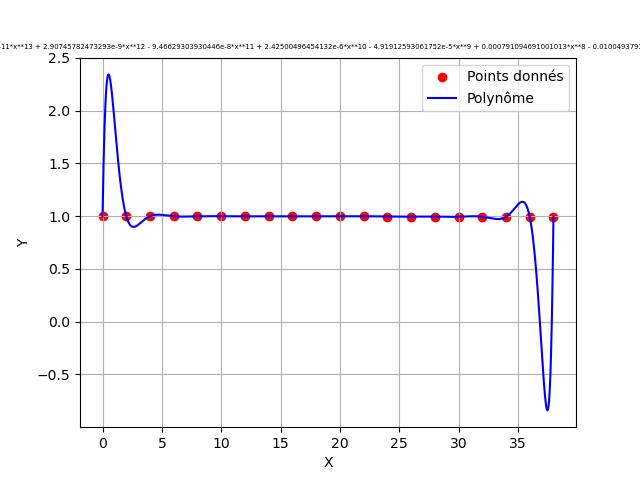
\includegraphics[width=0.7\textwidth]{sources/max/res41.-fig.png}
    \caption{Interpolation du jeu de données 1 de l'annexe}
\end{figure}
\newpage
\begin{lstlisting}[caption=res42.err, basicstyle=\fontsize{8}{10}\selectfont]
2.458392e+20 x**0 -6.969795e+18 x**1 
9.358358e+16 x**2 -7.912985e+14 x**3 
4.725728e+12 x**4 -2.118969e+10 x**5 
7.402081e+07 x**6 -2.062875e+05 x**7 
4.658351e+02 x**8 -8.608161e-01 x**9 
1.308859e-03 x**10 -1.640429e-06 x**11 
1.691843e-09 x**12 -1.428068e-12 x**13 
9.769647e-16 x**14 -5.333753e-19 x**15 
2.269488e-22 x**16 -7.253557e-26 x**17 
1.638308e-29 x**18 -2.331672e-33 x**19 
1.572710e-37 x**20 
runtime: 0.000459 seconds
sympy:
1.57271e-37*x**19 - 2.214532951e-33*x**18 
+ 1.4733504470928e-29*x**17 - 6.15598452675997e-26*x**16 
+ 1.81085839954286e-22*x**15 - 3.98452585608767e-19*x**14 
+ 6.8006270504217e-16*x**13 - 9.2128735250787e-13*x**12 
+ 1.00524804614512e-9*x**11 - 8.91203913542775e-7*x**10 
+ 0.00064458235891123*x**9 - 0.380327915947197*x**8 
+ 182.308394414935*x**7 - 70370.74352899*x**6 
+ 21553545.6995935*x**5 - 5118647118.33503*x**4 
+ 908843928869.321*x**3 - 113546693973050.0*x**2 
+ 8.90320254837454e+15*x - 3.29603172723061e+17
\end{lstlisting}
\begin{figure}[h]
    \centering
    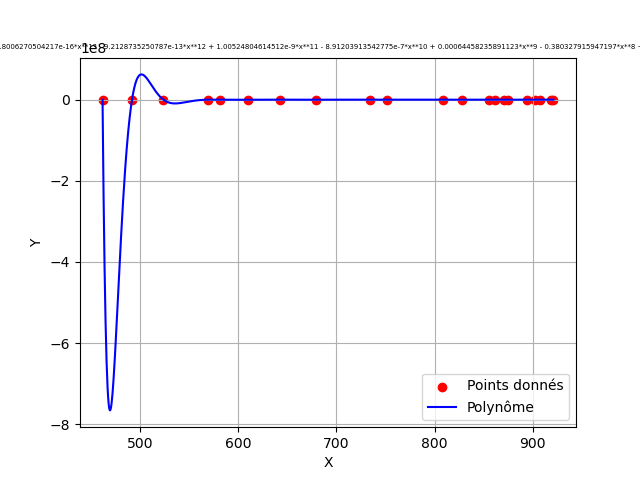
\includegraphics[width=0.7\textwidth]{sources/max/res42.-fig.png}
    \caption{Interpolation du jeu de données 2 de l'annexe}
\end{figure}
\newpage
\begin{lstlisting}[caption=res43.err, basicstyle=\fontsize{8}{10}\selectfont]
4.256997e+04 x**0 -5.137055e+04 x**1 
2.718367e+04 x**2 -8.326764e+03 x**3 
1.639873e+03 x**4 -2.176697e+02 x**5 
1.978914e+01 x**6 -1.220950e+00 x**7 
4.908433e-02 x**8 -1.164297e-03 x**9 
1.240079e-05 x**10 
runtime: 0.000370 seconds
sympy:
1.240079e-5*x**9 - 0.0009920632*x**8 
+ 0.034549978806*x**7 - 0.686034520134*x**6 
+ 8.539600378064*x**5 - 68.950370431266*x**4 
+ 360.417137962484*x**3 - 1174.64043365198*x**2 
+ 2165.03144523226*x - 1720.15728683702
\end{lstlisting}
\begin{figure}[h]
    \centering
    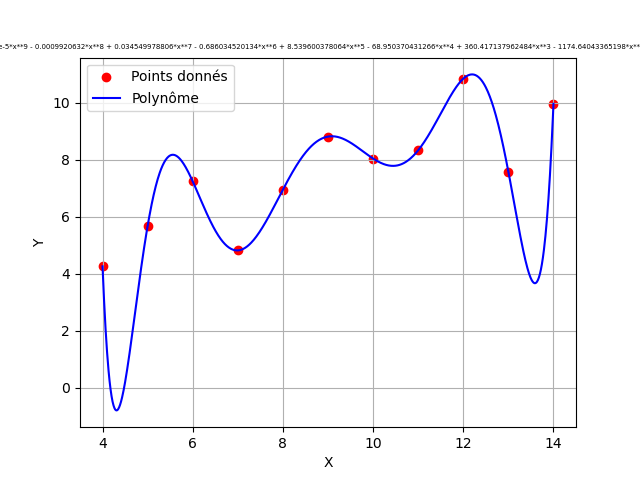
\includegraphics[width=0.7\textwidth]{sources/max/res43.-fig.png}
    \caption{Interpolation du jeu de données 3 de l'annexe}
\end{figure}
\newpage
\begin{lstlisting}[caption=res44.err ,basicstyle=\fontsize{8}{10}\selectfont]
4.256997e+04 x**0 -5.137055e+04 x**1 2.718367e+04 x**2 
-8.326764e+03 x**3 1.639873e+03 x**4 -2.176697e+02 x**5 
1.978914e+01 x**6 -1.220950e+00 x**7 4.908433e-02 x**8 
-1.164297e-03 x**9 1.240079e-05 x**10 
runtime: 0.000363 seconds
sympy:
1.240079e-5*x**9 - 0.0009920632*x**8 
+ 0.034549978806*x**7 - 0.686034520134*x**6 
+ 8.539600378064*x**5 - 68.950370431266*x**4 
+ 360.417137962484*x**3 - 1174.64043365198*x**2 
+ 2165.03144523226*x - 1720.15728683702
\end{lstlisting}
\begin{figure}[h]
    \centering
    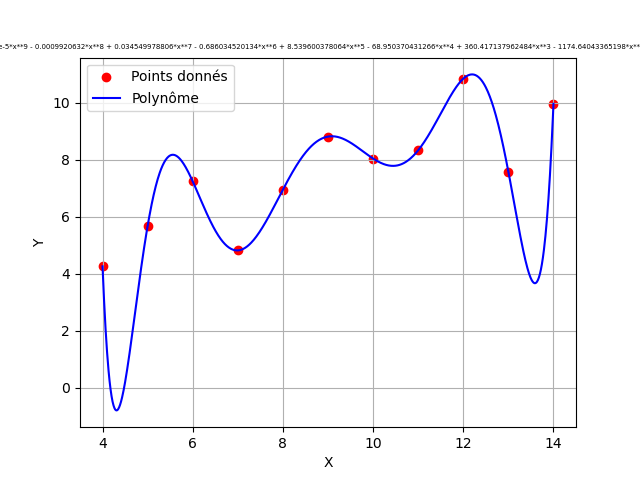
\includegraphics[width=0.7\textwidth]{sources/max/res44.-fig.png}
    \caption{Interpolation du jeu de données 4 de l'annexe}
\end{figure}